\documentclass[a4paper, fontsize=12pt, ngerman, oneside, openright]{scrreprt}

% Rendering packages
\usepackage{amsmath}
\usepackage{amssymb}
%\usepackage[draft]{graphicx}
\usepackage{graphicx}
\usepackage{wrapfig}
\usepackage{svg}
\usepackage{subcaption}
\usepackage{placeins}
\usepackage{xcolor}      % use if color is used in text
\usepackage{eurosym}
\usepackage{float}
\usepackage[toc,page]{appendix}

% Page dimensions
\usepackage[inner=2.5cm,outer=2.5cm,top=3.7cm,bottom=3.5cm]{geometry} 
\usepackage{parskip}
\usepackage[onehalfspacing]{setspace}

% Font styling
\usepackage[english]{babel}
\usepackage[utf8]{inputenc}
\usepackage[T1]{fontenc}
\usepackage{lmodern}
\renewcommand\familydefault{\sfdefault}
\usepackage[11pt]{moresize}

% Tables
\usepackage{tabularx}
\usepackage{tabulary}
\usepackage{longtable, lscape}

% Headers
\usepackage{scrpage2}  % header and footer for KOMA-Script
\pagestyle{scrheadings}
\automark[section]{chapter}

% Zitate
\usepackage[backend=biber, 
			style=authoryear,
			isbn=false, 
			sorting=nyt,
			]{biblatex}
\usepackage[babel,german=quotes, english=british, threshold=3]{csquotes}
\bibliography{Bibliothek/Bibliothek}

\usepackage[hyperindex,breaklinks,colorlinks=true,linkcolor=black,urlcolor=blue,citecolor=black]{hyperref}

% Code Blöcke
\usepackage{listings}
%\usepackage{Header/listings-golang} % import this package after listings
\usepackage{syntax}



%\lstset{ % add your own preferences
%	frame=single,
%	captionpos=b,
%	mathescape=true,
%	basicstyle=\footnotesize\ttfamily,
%	keywordstyle=\color{black},
%	numbers=left,
%	numbersep=5pt,
%	showstringspaces=false, 
%	stringstyle=\color{blue},
%	tabsize=2,
%	language=Golang % this is it !
%}


%table colors
\usepackage{xcolor,colortbl}

\newcommand{\mc}[2]{\multicolumn{#1}{c}{#2}}
\definecolor{Gray}{gray}{0.85}
\definecolor{LightCyan}{rgb}{0.88,1,1}

\newcolumntype{a}{>{\columncolor{Gray}}c}
\newcolumntype{b}{>{\columncolor{Gray}}l}

\usepackage{color}
\definecolor{gray}{rgb}{0.4,0.4,0.4}
\definecolor{darkblue}{rgb}{0.0,0.0,0.6}
\definecolor{cyan}{rgb}{0.0,0.6,0.6}
\definecolor{dkgreen}{rgb}{0,0.6,0}
\definecolor{gray}{rgb}{0.5,0.5,0.5}
\definecolor{mauve}{rgb}{0.58,0,0.82}


\lstset{frame=tb,
	language=Java,
	aboveskip=3mm,
	belowskip=3mm,
	showstringspaces=false,
	columns=flexible,
	basicstyle={\small\ttfamily},
	numbers=none,
	numberstyle=\tiny\color{gray},
	keywordstyle=\color{blue},
	commentstyle=\color{dkgreen},
	stringstyle=\color{mauve},
	breaklines=true,
	breakatwhitespace=true,
	tabsize=3
}

\lstdefinelanguage{XML}
{
	morestring=[b]",
	morestring=[s]{>}{<},
	morecomment=[s]{<?}{?>},
	morecomment=[s]{!--}{--},
	stringstyle=\color{black},
	identifierstyle=\color{darkblue},
	keywordstyle=\color{cyan} list your attributes here
}

%pdf insert
\usepackage{pdfpages}

%zusätzliche Trennungen
\hyphenation{Grund-ar-chi-tek-tur}
\hyphenation{MQTT-Kom-mu-ni-ka-tions-mo-dell}
\hyphenation{Master-Master-Replikation}
\hyphenation{Pub-lish-er}
\hyphenation{Pub-lish-ers}
\hyphenation{Sub-scriber}
\hyphenation{Sub-scribers}
\hyphenation{Pub-lish er/Sub-scriber}
\hyphenation{beo-bacht-bar}
\hyphenation{Score}
\hyphenation{Ac-knowl-edge-ment}
\hyphenation{Ac-knowl-edge-ments}

\usepackage{mathtools}
\DeclarePairedDelimiter\abs{\lvert}{\rvert}

\usepackage{acronym}



\begin{document}

% Titelseite einfügen.
\begin{titlepage}


\begin{center}
 		
\includegraphics[scale=1]{Resources/Haw}
\end{center}

\begin{center}
	\HUGE \textbf{Title}
	\large\\Subtitle\\ \ \\
	\small SubSubtitle \\
	SS 2018 - WS 2018/2019
\end{center}

\begin{center}
Authors
\end{center}

\end{titlepage}

\clearpage

% Counter zurücksetzen. Römische Ziffern einstellen.
\pagenumbering{Roman}
\setcounter{page}{1}

% Inhaltsverzeichnis generieren.
\tableofcontents

% Neue Seite. Counter zurücksetzen. Arabische Ziffern einstellen.
\clearpage
\pagenumbering{arabic}
\setcounter{page}{1}

% Kapitel einfügen.
\chapter{Geschichte}
\section{Industrieroboter}
Nach Definition der VDI-Richtlinie 2860 sind Industrieroboter universell einsetzbare Bewegungsautomaten mit meherern Achsen, deren Bewegungen hinsichtlich Bewegungsfolge und Wegen bzw. Winkel frei programmierbar und sensorgeführt sind.
\begin{itemize}
	\item Zeichnen sich durch \textbf{Schnelligkeit}, \textbf{Genauigkeit}, \textbf{Robustheit }und eine hohe \textbf{Traglast }aus.
	\item Einsatzgebiete: Schweißen, Kleben, Schneide, Lackieren
\end{itemize}
Zunehmend \textbf{kollaborative} Roboter, Cobots:
\begin{itemize}
	\item Industrieroboter, die mit Menschen gemeinsam arbeiten
	\item Nicht mehr durch Schutzeinrichtungen im Produktionsprozess von Menschen getrennt
	\item Nimmt Menschen wahr, verursacht keine Verletzungen
\end{itemize}

\section{Serviceroboter}
\subsection{Definition}
\begin{itemize}
	\item Ein \textbf{Serviceroboter} ist eine \textbf{frei programmierbare Bewegungseinrichtung}, die \textbf{teil- oder vollautomatisch} Dienstleistungen verrichtet.
	\item \textbf{Dienstleistungen} sind dabei Tätigkeiten, die nicht der direkten industriellen ERzeugung von Sachgütern, sondern der Verrichtung von \textbf{Leistungen für Menschen und Einrichtungen} dienen.
	\item Einteilung in zwei Klassen
	
\end{itemize}
\subsection{Klassen}
\begin{itemize}
	\item Roboter, die für professionellen Einsatzbereich: \textbf{Rettung}, \textbf{Landwirtschaft}, \textbf{Medizin}
	\item Roboter für den Privaten gebrauch: \textbf{Staubsauger}, \textbf{Rasenmäher}, \textbf{Pfleger}
\end{itemize}
\chapter{Software-Architekturen für mobile Robotersysteme}
\section{Probleme und Anforderungen}
\subsection{Definition mobile Roboter}
\enquote{Unter einem Roboter verstehen wir eine frei programmierbare Maschine, die auf Basis von Umgebungssensordaten in geschlossener Regelung in Umgebungen agiert, die zur Zeit der Programmierung nicht genau bekannt und/oder dynamisch und oder nicht vollständig erfassbar sind.}
$\Rightarrow$ \textbf{Joachim Herzberg, Mobile Roboter}
\subsection{Umgebung mobiler Roboter}
Bei \textbf{mobilen Robtoern} ist die Umgebung im Detail \textbf{nicht bekannt und generell nicht kontrollierbar}
\begin{itemize}
	\item Alle Aktionen sind von der aktuellen Umgebung abhängig
	\item Details sind erst zum Zeitpunkt der Ausführung der Aktionen bekannt
	\item Mobile Roboter müssen in einer geschlossenen Regelung
		\subitem die Umgebung mit Sensoren erfassen
		\subitem die Daten auswerten
		\subitem Aktionen daraus planen
		\subitem Aktionen mittels Koordination der Aktuatoren umsetzen
\end{itemize}
\subsection{Roboterkontroll-Architekturen}
\paragraph{Herausforderungen}
\begin{itemize}
	\item Robotersystem besteht aus den Gebieten \textbf{Wahrnehmung}, \textbf{Planung} und \textbf{Handlung}
	\item Herausforderungen an eine Roboterkontroll-Architektur, sie muss:
	\subitem Sensorwerte erfassen und auswerten
	\subitem Pfade planen
	\subitem Hindernisse vermeiden
	\subitem Komplexe Algorithmen in langen Zeitzyklen ausführen
\end{itemize}
\paragraph{Probleme bei der Software-Erstellung zur Roboterkontrolle}
\begin{itemize}
	\item Roboter sind eingebettete Systeme, die in geschlossener Regelung laufen und die Sensorströme in \textbf{Echtzeit verarbeiten} müssen
	\item Untschiedliche Aufgaben --> Unterschiedliche Zeitzyklen
	\item Unterschiedlicher Zeitskalen --> kein standardisierter Kontroll- oder Datenfluss den die Architektur abbilden könnten
	\item Für etliche algorithmische Teilprobleme sind \textbf{keine effizienten Verfahren} bekannt
	\item \textbf{Prozessorkapazität ist begrenzt}
\end{itemize}
\subsection{Anforderungen an das Kontrollsystem eines autonomen Roboters}
\paragraph{Robustheit}
\begin{itemize}
	\item Die Umgebung des Systems kann sich ständig ändern
	\item Auf eine Umgebungsänderung sollte der Roboter sinnvoll reagieren und nicht verwirrt stehen bleiben.
	\item Verwendete Modelle der Umgebung sind ungenau.
\end{itemize}
\paragraph{Unterschiedliche Ziele}
\begin{itemize}
	\item Der Roboter verfolgt zu einem Zeitpunkt eventuell Ziele, die im Konflikt zueinander stehen.
	\item \textbf{Beispiel}: der Roboter soll ein bestimmtes Ziel ansteuern, dabei aber Hindernissen ausweichen.
\end{itemize}
\paragraph{Sensorwerte von mehreren Sensoren}
\begin{itemize}
	\item Sensordaten könen verrauscht sein
	\item Sensoren können fehlerhafte oder inkonsistente Messwerte liefern, weil der Sensor z.B. außerhalb seines Bereichs misst für den er zuständig ist und dies nicht überprüfen kann.
\end{itemize}
\paragraph{Erweiterbarkeit}
\begin{itemize}
	\item Wenn der Roboter neue Sensoren erhält, sollte dies leicht in das Programm integriert werden können.
\end{itemize}
\section{Mögliche Modelle}
\subsection{Klassisches Modell - der funktionale Ansatz}
Das \textbf{klassische Model} wird auch als hierarchisches Model oder funktionales Model bezeichnet.
Ist ein Top-Down Ansatz, besteht aus drei Abstraktionsebenen
\begin{itemize}
	\item Die unterste Ebene: \textbf{Pilot}
	\item Mittlere Eben: \textbf{Navigator}
	\item Oberste Ebene: \textbf{Planer}
\end{itemize}
\textbf{Sense-Think-Act-Cycle} oder \textbf{SMPA} (Sense - Model - Plan - Act).
\begin{itemize}
	\item Sensordaten, die vom Fahrzeut geliefert werden, werden in den zwei unteren Ebenen vorverarbeitet.
	\item Konstruktion oder Aktualisierung eines Weltmodells
	\item \textbf{Planer} ist die Basis aller Entscheidungen basieren auf dem zugrundelgenden Weltmodell
	\item Tatsächliche Fahrbefehle werden durch unterste Ebene ausgeführt
\end{itemize}
Zyklus wird ständig wiederholt $\Rightarrow$ wenn alle Ebenen richtig funktionieren resultiert daraus ein intelligentes Verhalten und die Erfüllung der Aufgabe.
\paragraph{Nachteile}
\begin{itemize}
	\item \textbf{Sequentieller Ansatz}, \textbf{lange Kontrollzykluszeit}
	\item Gesamtsystem anfällig, $\Rightarrow$ fällt ein Modul scheitert das Gesamtsystem
	\item Die Repräsentation der Umgebung muss alle notwendigen Informationen enthalten, damit ein Plan entwickelt werden kann.
	Planer hat nur Zugriff auf das Weltmodell $\Rightarrow$ während Planer aktionen ausarbeitet, könnte sich die Umwelt schon wieder geändert haben.
\end{itemize}
\subsection{Verhaltensbasiertes Modell}
\paragraph{Grundlegender Gedanke} Intelligentes Verhalten wwird nicht durch komplexe, monolithische Kontrollstrukturen erzeugt, sondern durch das Zusammenführen der richtigen einfachen Verhalten und deren Interaktion.
\paragraph{Definition}
\begin{itemize}
	\item Engere Verbindung zwischen \textbf{Wahrnehmung} und \textbf{Aktion}
	\item Jede \textbf{Roboterfunktionalität} wird in einem \textbf{Behavior} gekapselt
	\item Alle \textbf{Behaviors} werden \textbf{parallel ausgeführt}
	\item Jedes Behavior Modul operiert unabhängig von den anderen
	\item Alle Behaviors können auf alle Fahrzeugsensoren zugreifen und gewissermaßen die Aktuatoren ansteuern.
\end{itemize}
\paragraph{Beispiel}
\textbf{Subsumption Architektur nach Brooks}
\newpage
\subsection{Hybrider Ansatz}
\begin{itemize}
	\item Nutzt die Vorteile der \textbf{Subsumption Architektur} und der \textbf{SMPA-Architektur}
	\item Der verhaltensbasierte Anteil ist nicht geeignet, auf längere Sicht zielgerichtet Aktionen zu koordinieren $\Rightarrow$ SMPA-Anteil
\end{itemize}
\begin{figure}[H]
	\begin{center}
		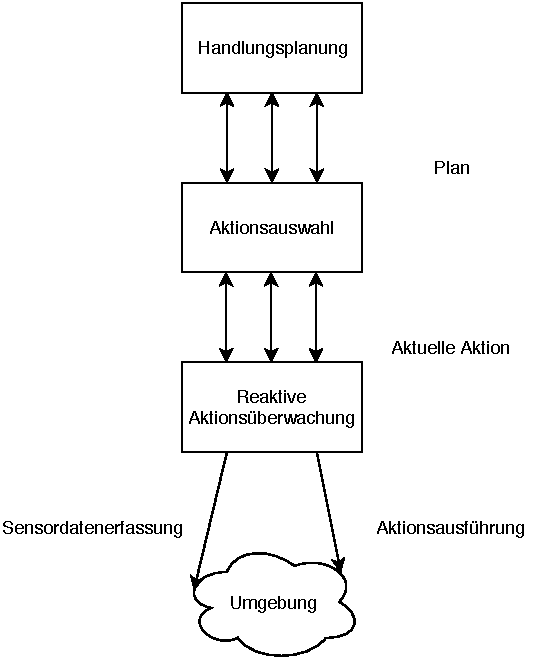
\includegraphics[scale=0.9]{Resources/PDF/HybridModel}
		\caption{Schema der Hybridmodell Schichten}
		\label{fig:PDF/HybridModel}
	\end{center}
\end{figure}
\begin{itemize}
	\item Die \textbf{Handlungsplanung} arbeitet auf hoher, strategischer Stufe in langen Zeitzyklen
	\item Die \textbf{reaktive Aktionsüberwachung} enthält die Verhaltensbausteine auf operativer Ebene, die in schellen Zeitzyklen die physische Roboteraktion anstoßen und überwachen
	\item die \textbf{mittlere Kontrollebene} hat die taktische Aufgabe, die jeweils \textbf{nächste Aktion aus dem Plan auszusuchen} zu instanzieren und auf die Ebene der Verhaltensbausteine zu zerlegen
	Des weiteren muss die die Rückmeldung von der Aktionsüberwachung interpretieren und entscheiden ob eine Aktion erfolgreich abgeschlossen ist. $\Rightarrow$ entscheiden ob die Handlungsplanung einen anderen Plan erstellen muss
\end{itemize}
\newpage
\paragraph{Kritik}
\begin{itemize}
	\item Mittlere Komponente benötigt den größten konzeptuellen und programmiertechnischen Aufwand
	\item Das mittlere Teilproblem ist deutlich komplexer als die beiden anderen
\end{itemize}
\subsection{Probabilistische Robotik}
\begin{itemize}
	\item Probabilistische Robotik berücksichtigt die \textbf{Unsicherheit der Wahrnehmund und der Aktionen}
	\item \textbf{Schlüsselidee} Information in Form von Wahrscheinlichkeitsdichten repräsentieren
	\item Eine Lokalisierung der Roboter wird unter Verwendung von wahrscheinlichkeitstheorie oder einer Wahrscheinlichkeitsverteilung eine Aussage über die Umgebung treffen
	\item \textbf{Probabilistische Wahrnehmung}: wenn man Sensorwerte schätzen kann, dann kann man mit Wahrscheinlichkeitstheorie/Wahscheinlichkeitsverteilung eine Aussage über die Umgebung treffen
	\item \textbf{Probabilistisches Handeln}: aufgrund der Unsicherheit über die Umgebung ist auch das Handeln mit Unsicherheit behaftet.
	Mit probabilistischen Ansätzen besteht die Möglichkeit Entscheidungen trotz Unsicherheit zu treffen
\end{itemize}
\paragraph{Vorteil} probabilistische Verfahren können auch mit weniger präzisen Umgebungsmodellen angewandt werden.
\paragraph{Nachteil} weniger effizient wegen komplexer Berechnungen, Approximation erforderlich
\subsection{Subsumption-Architektur in Bezug auf die Anforderungen des Robotersteuerungssystems}
\paragraph{Robustheit}
\begin{itemize}
	\item Wenn einige Steuerungsmodule ausfallen, arbeiten bei der Subsumption-Architektur in die restlichen Schichten einwandfrei $\Rightarrow$ \textbf{eingeschränktes, aber sinnvolles Verhalten möglich}
\end{itemize}
\paragraph{Unterschiedliche Ziele}
\begin{itemize}
	\item Mehrere Teilsituation können verschiedene Verhaltenselemente sinvoll machen, die sich widersprechen können.
	\item Die Wichtigkeit einer Handlung hängt vom Kontext ab, d.h. höhere Ziele können niederere Ziele ersetzen.
	\item Alle zu einem Zeitpunkt möglichen Verhaltenselemente werden parallel bearbeitet.
	\item Das \textbf{resultierende Verhalten wird in Abhängigkeit von Umwelteinflüssen dynamisch} bestimmt
	\item Das Gesamtergebnis hängt nicht von einer übergeordneten Instanz ab
\end{itemize}
\paragraph{Sensorwerte von mehreren Sensoren}
\begin{itemize}
	\item Der Roboter muss auch bei inkonsistenten Informationen eine Entscheidung fällen
	\item Die Subsumption-Architektur sieht keine zentrale Verarbeitung und Speichung der Umweltdaten
	\item Jedes Modul reagiert nur auf die Daten einzelner Sensoren, es muss \textbf{kein konsistentes Abbild der Umwelt erschaffen werden}
\end{itemize}
\paragraph{Erweiterbarkeit}
Das bestehende Verhalten kann jederzeit durch Hinzufügen weiterer Schichten um komplexere Funktionen erweitert werden
\section{ROS - Robot Operating System}
\subsection{Entwicklung}
\begin{itemize}
	\item \textbf{Das Architekturschema für Roboterkontrollsoftware} gibt es nicht $\Rightarrow$ deshalb heute auch Unterstützung der Roboter-Softwareentwicklung durch Middleware wie ROS
	\item \textbf{Zweck}: soll die Entwicklung von Software für Roboter vereinfachen und wiederkehrende Aufgaben standardisieren
	\item Standard für Robotoerkontrollsoftware
\end{itemize}
\subsection{Design Prinzipien}
\begin{figure}[H]
	\begin{center}
		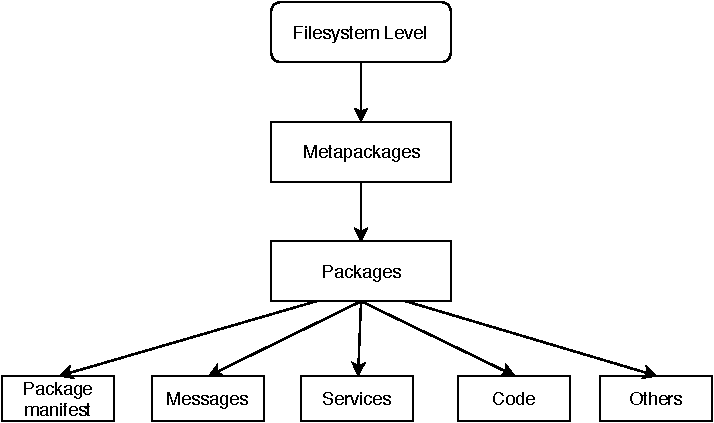
\includegraphics[]{Resources/PDF/FileSystem}
		\caption{Filesystem, das ROS zugrunde liegt}
		\label{fig:PDF/FileSystem}
	\end{center}
\end{figure}
\begin{itemize}
	\item Ein Package beinhaltet die ROS Prozesse, welche auch Nodes genannt werden
	\item Komplexe Prozesse werden durch Netzwerke von Nodes bewerkstelligt
	\item Roboterkontrollprogramm besteht aus vielen Prozessen, die potentiell über mehrere Rechner verteilt sein können
	\item Wichtigster Knoten ist der Master $\Rightarrow$ Abwicklung der internen Kommunikation
	\item Andere Knoten können nur starten, wenn ein Master existiert
	\item Nodes müssen sich beim Master anmelden
	\item Funktionalität (Kommandods, Ausführung v. Algorithemen) wird in eigenen Nodes realisiert
	\item Nodes sind in verschiedene Prozesse getrennt $\Rightarrow$ fehlerhafte Knoten hat i.d. Regel wenig Auswirkungen auf die anderen
	\item Knoten werden über Publish-Subscribe verknüpft
	\item \textbf{Asynchrone Nachrichten} werden durch Topics ausgetauscht
	\item \textbf{Synchrone Nachrichten} werden durch Services ausgetauscht
\end{itemize}
\subsection{Publish - Subscribe}
\paragraph{Nodes} sind Software-Module, die die Verarbeitung durchführen. Sie kommunizieren über Topics miteinander und tauschen dabei Nachrichten.
\paragraph{Kommunikation}
Die Kommunikation basiert auf einem \textbf{Publish Subscribe Pattern}
\begin{itemize}
	\item Wenn Daten weitergegeben werden sollen, wird ein Publisher erzeugt
	\item Publisher registriert sich beim Master und gibt Topics an
	\item Daten können in anderen Knoten abgerufen werden -- dazu wird ein (oder mehrere) Subscriber angelegt
	\item Subscriber frägt beim Master bezüglich gewünschten Topics an
	\item Daten werden über TCP/IP Sockets übertragen
\end{itemize}
\paragraph{Topics}
\begin{itemize}
	\item Themen, zu denen die Nodes Messages versenden
	\item Topics sind einfach Strings
	\item Verschiedene Nodes können zu einem bestimmten Topic Nachrichten versenden
	\item Ein Node kann sich prinzipiell zu mehreren Topics einschreiben und mehrere Topics publizieren
\end{itemize}
\paragraph{Services}
\begin{itemize}
	\item Nachteil von Publish Subscribe wird durch Services geschlossen
	\item Sind eine weitere Art, wie Nodes kommunizieren können
	\item Synchroner Nachrichtenaustausch mithilfe von Requests, welche von anderen Nodes mit einer Response beantwortet werden
	\item Ein Knoten registriert eine Aktion (Service), namentlich beim Master
	\item Ein Service Caller kann die Ausführung eines Services anstoßen, sobald dieser verfügbar ist
	\item geeignet für RMI oder einmalige Anfragen
\end{itemize}
\paragraph{Messages}
\begin{itemize}
	\item werden von Nodes bei der Kommunikation
	\item Messages sind streng typisierte, möglicherweise verschachtelte Datenstrukturen, die aus den primitiven Typen int, float, bool bestehen
	\item Eine Message kann andere Messages oder Felder von Messages enthalten
\end{itemize}
%seite 25 kapitel 2
\chapter{Lokalisation autonomer mobiler Robotersysteme}
\section{Abgrenzung: Lokalisation - Mapping - SLAM - Navigation}
\begin{itemize}
	\item \textbf{Lokalisation} Ermitteln der aktuellen Position des Roboters.
	\item \textbf{Kartenerstellung, Mapping oder Umgebungsmodellierung} hilft bei Entscheidung
	\subitem Kartenerstellung bedeuted die Auswertung der vom Roboter mittels Sensoren erfassten Daten der Umgebung mit dem Ziel, ein Umgebungsmodell zu erzeugne oder zu vervollständigen.
	\item \textbf{Großes Problem} Mapping
	\item \textbf{Pfadplanung oder Navigation} beantwortet die Frage \textbf{Wie gelange ich dorthin?} Bewegungsplanung oder Pfadplanung bedeutet die Berechnung der Fahrroute und der daraus abgeleiteten Bahn vom aktuellen Punkt zum Zielpunkt
	\item Man unterscheidet zwischen Navigation in unbekannter und in bekannter Umgebung.
	\item Selbstlokalisation und Kartenerstellung bedingen sich gegenseitig.
\end{itemize}
\section{Varianten der Selbstlokalisierung}
\paragraph{Lokale Selbstlokalisierung (position tracking)}
\begin{itemize}
	\item Die Startposition des Roboters ist ungefähr bekannt.
	\item Es handelt sich um \textbf{relative} Selbstlokalisierung
	\item Sobald sich der Roboter bewegt, muss aufgrund neuer Sensordaten die Position neu berechnet werden.
	\item Bezugspunkt ist der Startpunkt.
	\item \textbf{Methoden} Odometrie und Trägheitsnavigation
\end{itemize}
\paragraph{Globale Selbstlokalisierung}
\begin{itemize}
	\item Die Startposition ist unbekannt.
	\item Es handelt sich um \textbf{absolute Positionierung}
	\item An welcher Position der Roboter befindet, entscheidet er durch Auswerten seiner Sensordaten und durch erkennen von \textbf{signifikanten} Umgebungsmerkmalen
	\item \textbf{Mögliche Methode}: Triangulation
\end{itemize}
\paragraph{Kidnapped Robot Problem}
\begin{itemize}
	\item Die Position des Roboters ist anfangs bekannt
	\item Der Roboter wird willkürlich mit temporär deaktivierten Sensoren an eine beliebige andere Position versetzt, ohne darüber informiert zu werden.
	\item Auch dann muss das Verfahren robust die Position wiederfinden, zunächst muss der Roboter dies erkennen und sich dann relokalisieren
	\item Es muss eine erneute globale Lokalisierung durchgeführt werden
\end{itemize}
\section{Relative Lokalisierung versus Absolute Lokalisierung}
\paragraph{Relative Lokalisierung}
\begin{itemize}
	\item auch: \textbf{lokale}, \textbf{inkrementelle Lokalisierung} oder \enquote{tracking}
	\item Relativ zu einer Startpose wird sukzessiv die Änderung der Pose an diskreten, aufeinanderfolgenden Zeitpunkten ermittelt und integriert
\end{itemize}
\paragraph{Absolute Lokalisierung}
\begin{itemize}
	\item auch als \textbf{globale Lokalisierung} bezeichnet
	\item Die Pose wird in Bezug auf ein externes Bezugssystem ermittelt, z.B. einer Karte oder einem globalen Koordinatensystem
\end{itemize}
\paragraph{Ziel} Bestimme oder schätze die Position und Orientierung des Roboters in seiner Umgebung basieren auf
\begin{itemize}
	\item der Eigenbewegung
	\item durch Messungen der relativen Position zu unterscheidbaren Objekten in der Umgebung in Roboterkoordinaten (Ultraschall, Laser, Kamera)
\end{itemize}
%BSP Chapter 3 Seite 4 / 28 
\section{Transformation von Koordinatensystemen lokale <--> globale}
\paragraph{Kinematik} Die Kinematik ist die Lehre der Beschreibung von Bewegungen von Punkten im Raum. Dabei werden die Größen Weg, Geschwindigkeit und Beschleunigung betrachtet. Die Kinematik ist ein Teilgebiet der Mechanik.
\paragraph{Kinematische Robotermodell}
\begin{itemize}
	\item kreisförmiger Roboter
	\item Zweiradantrieb
	\item Bewegung in der Ebene
\end{itemize}
\paragraph{Lokales Koordinatensystem}
\begin{itemize}
	\item mit dem Roboter verbunden
	\item Ursprung in der Mitte der Antriebsachse
	\item x-Achse zeigt in Richtung des Roboterfrontteils
\end{itemize}
\paragraph{Festlegung der Roboterposition im globalen Koordinatensystem}
\begin{itemize}
	\item durch die Koordinaten $M(x_{M}, y_{M})$ im globalen Koordinatensystem
	\item durch den Winkel $\theta$ zwischen der lokalen x-Achse und der globalen x-Achse
	\item Pose p gegeben durch: p = $(x_M, y_M, \theta)^{T}$
\end{itemize}
\paragraph{Transformation von lokalen in globale Koordinaten}
\begin{itemize}
	\item Koordinaten von P im lokalen Koordinatensystem: $p_l=(x_l, y_l)^T$
	\item Koordinaten von P im globalen Koordinatensystem: $p_g = (x_g, y_g)^T$
	\item Transformation von $p_l$ nach $p_g(m=(x_M, y_M)^T: p_g=R(\theta)p_l)$
\end{itemize}
\paragraph{Transformation von globalen in lokale Koordinaten}
\begin{itemize}
	\item Transformation von globalen in lokale Koordinaten $p_l = R(\theta)^-1(p_g - m) = R(-\theta)(pg - m)$
\end{itemize}
\section{Karten für statistische und dynamische Umgebungen}
\begin{itemize}
	\item Generell gilt: \textbf{Karten} sollen eine explizite Repräsentation des Raumes sein.
	\item Die Karten sind auf die Sensorik des Roboters zugeschnitten
	\item Die Karten sind nicht vorrangig für den menschlichen Betrachter bestimmt, sondern der Roboter soll sie effizient nutzen können.
\end{itemize}
\paragraph{Statische Umgebungen}
\begin{itemize}
	\item basierend auf der Annahme, dass sich zwar der Zustand des Roboters innerhalb der Umgebung, nicht jedoch die Umgebung selbst ändert.
	\item Karte spiegelt die wirkliche Umgebung wider.
\end{itemize}
\paragraph{Dynamische Umgebungen}
\begin{itemize}
	\item Objekte können ihre Lage oder ihren Zustand ändern
	\item In der Karte registrierte Objekte können verschwinden, nicht registrierte Objekte auftauchen
	\item \enquote{Lernende} Karten sind ein fundamentales Problem in der mobilen Robotik
\end{itemize}
\subsection{Mapping Methoden}
\paragraph{Weltzentriert}
\begin{itemize}
	\item Die Pose aller Objekte einschließlich des Roboters werden in der Umgebung in Bezug auf ein festes Koordinatensystem repräsentiert.
	\item \textbf{Indoor}: Ursprung kann eine Zimmerecke sein
	\item \textbf{Outdoor}: Benötigung eines globalen Koordinatensystems, wie z.B. die Längen- oder Breitengrade, i.d.R. nutzen von \textbf{WGRS}(World Geographic Reference System)
\end{itemize}
\paragraph{Roboterzentriert} gebraucht um bspw. Kollisionen zu vermeiden
\begin{itemize}
	\item Durch Koordinaten-Transformation kann zwischen den verschiedenen Referenz-Frames konvertiert werden
\end{itemize}
\subsection{Arten von Modellen}
\begin{itemize}
	\item Die wichtigste Form von Umgebungsmodellen für mobile Roboter sind Umgebungskarten.
	\item Die folgende Ausführungen beziehen sich auf geeignet Karten für \textbf{mobile, autonome Landfahrzeuge}
\end{itemize}
\begin{figure}[H]
	\begin{center}
		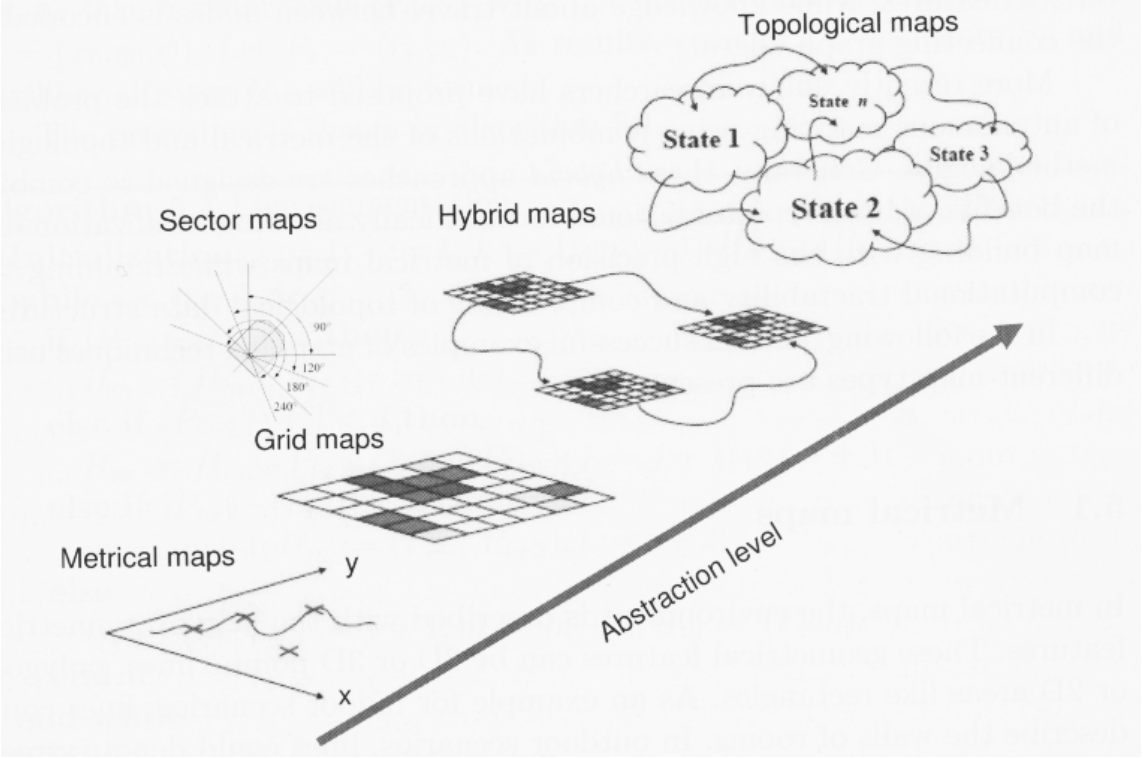
\includegraphics[scale=0.42]{Resources/PNG/MapTypes.PNG}
		\caption{}
		\label{fig:PNG/MapTypes.PNG}
	\end{center}
\end{figure}
\paragraph{Arten von Umgebungsmodellen}
\begin{itemize}
	\item \textbf{kontinuierliche metrische Karten}, zweidimensional oder dreidimensional:
	\subitem jedes Objekt wird assoziiert mit Koordinaten
	\item \textbf{diskrete metrische Karten, Grid Maps}, zweidimensional oder dreidimensional:
	\subitem der Raum wird gleichmäßig oder ungleichmäßig aufgeteilt; Objekte werden mit Positionen innerhalb des Gitters assoziiert
	\item \textbf{Hybrid Maps}
	\item \textbf{Topologische Modelle} nur zweidimensional
	\subitem im Vordergrund steht die Beziehung der Objekte zueinander
\end{itemize}
\subsection{Kontinuierliche Metrische Karten}
\begin{itemize}
	\item Metrische Lokalisierung, beruht auf Ultrashall oder Laserscannern
	\item Exakte Beschreibung der Umgebung mit 2D oder 3D Modellen möglich
	\item Die Positionen von Objekten der Umgebung werden durch ein Koordinatensystem repräsentiert.
	\item \textbf{Vorteil}: detailliertes Bild der Umgebung
	\item \textbf{Nachteil}: große, unstrukturierte Datenmengen erschweren die Pfadplanung
\end{itemize}
\subsection{Grid Maps - Rasterkarten}
\begin{itemize}
	\item Die Umwelt des Roboters wird in ein gleichmäßiges Raser oder Grid zerlegt.
	\item Jede Zelle enthält den Belegtheitsgrad der Zelle $\Rightarrow$ zeigt an ob zelle mit einem Hindernis belegt ist oder nicht
	\item Verschiedene Modelle verwenden unterschiedliche Werte
	\subitem zwei Werten
	\subitem freie Zellen, belegte Zellen und Zellen mit Mischbelegung
	\subitem Prozentsatz der Belegungswahrscheinlichkeit
	\item Notwendige Informatinoen sind z.B.:
	\subitem x, y als Koordinaten (Zeile, Spalte) einer Zelle
	\subitem Sensordaten des Roboters
	\subitem ein boolscher Wert für den Zustand der Zelle
	\item Die Werte in den Zellen sind unabhängig voneinander
	\item Eine Steigerung der Messgenauigkeit der Sensoren führt dazu, dass die Rasterelemente immer kleiner werden
	\item Für eine kompakte Notation können Grid Maps im 2-dimensionalen Raum mit Quadtrees im 3-dimensionalen mit Octtrees gespeichert werden
\end{itemize}
\paragraph{Gleichmäßige Gitterstruktur vs. Adaptiver Gitterstruktur}
\begin{figure}[H]
	\begin{center}
		\includegraphics[scale=0.5]{Resources/PNG/Quadtrees.PNG}
		\caption{}
		\label{fig:PNG/Quadtrees.PNG}
	\end{center}
\end{figure}
\begin{itemize}
	\item links oben zeigt die Objekte in einer gleichmäßigen Gitterstruktur
	\item rechts oben zeigt die zugehörige Repräsentation über Belegtheiten der Zellen
	\item speicherintensiv bei gleichmäßiger Unterteilung des Raums $\Rightarrow$ adaptive Unterteilung des Raums und Speicherung in Quadtrees oder bei 3. Dimension Octtrees
\end{itemize}
\subsection{Adaptive Unterteilung}
\begin{itemize}
	\item Ausgangszustand: Rechteck mit Hindernissen
	\item Fläche wird unterteilt in 4 Rechtecke gleicher Größe
	\item Jedes Rechteck wird rekursiv wieder in 4 Rechtecke unterteilt $\Rightarrow$ Quadtree
	\item Attributierung der Knoten:
	\subitem \textbf{Frei}: Rechteck enthält keinen Teil eines Hindernisses
	\subitem \textbf{Belegt}: Rechteck ist vollständig von Hindernis belegt
	\subitem \textbf{Gemischt}: Rechteck enthält Punkte, die zu einem Hindernis gehören, sowie solche die es nicht tun
	\item Nur gemischte Knoten werden weiter unterteilt
\end{itemize}
\paragraph{Vorteile} schnell und leicht feststellbar, ob Punkt in einem Hindernis liegt
\paragraph{Nachteile} 
\begin{itemize}
	\item Konturen der Objekte und der Freiraum zwischen ihnen wird unpräzise repräsentiert
	\item Um die Datenfülle zu reduzieren, wird das Raster zu grob gewählt und dadurch ein möglicher Weg durch Mischpixel versperrt
\end{itemize}
\paragraph{Weiterer Verwendungszweck}
Neben der reinen Lokalisierung können die Karten auch dazu verwendet werden eine Fahrspur (Trakektorie) zu berechnen.
\begin{figure}[H]
	\begin{center}
		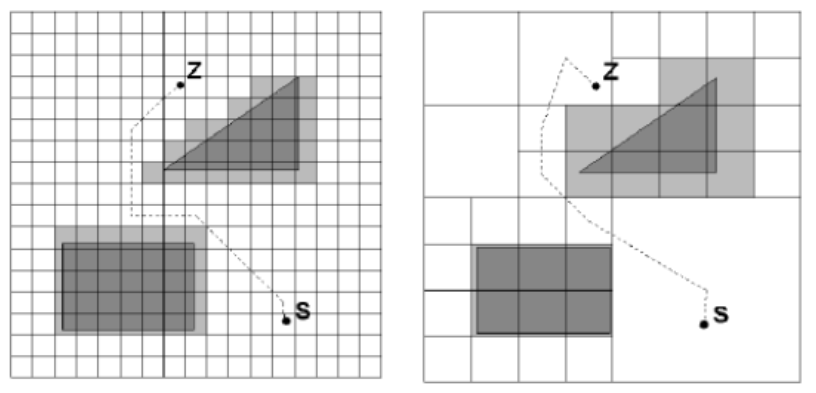
\includegraphics[scale=0.5]{Resources/PNG/Trajektorie}
		\caption{}
		\label{fig:PNG/Trajektorie}
	\end{center}
\end{figure}
\subsection{Weitere Beispiele für Umgebungskarten}
\begin{itemize}
	\item Laserscan Karten
	\item Bildbasierte Karten
\end{itemize}
\subsection{Topologische Karten}
Bedingt geeignet zur Lokalisation, Haupteinsatzgebiet ist die Pfadplanung.
\begin{figure}[H]
	\begin{center}
		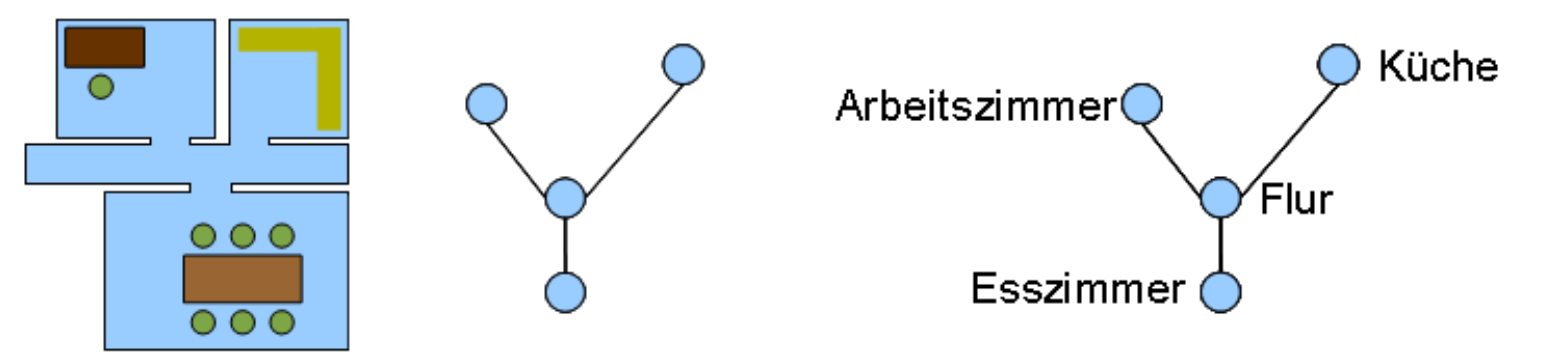
\includegraphics[scale=0.42]{Resources/PNG/TopologischeKarte.PNG}
		\caption{}
		\label{fig:PNG/TopologischeKarte.PNG}
	\end{center}
\end{figure}
\begin{itemize}
	\item Modelle bilden einen \textbf{Graphen}
	\item \textbf{Knoten} entsprechen Orten oder Bereichen der Umgebung
	\item Beziehungen zwischen den Orten werden durch \textbf{Kanten} modelliert.
	\item Zwei Knoten sind durch eine Kante verbunden, wenn sie unmittelbar voneinander erreichbar sind.
	\item \textbf{Gewichte}: Maß für die Länge der Wege
	\item Ist die Länge der jeweiligen Wegstücke bekannt, lässt sich der kürzeste Weg finden.
\end{itemize}
\paragraph{Vorteile}
\begin{itemize}
	\item Kompaktheit
	\item Gute Skalierbarkeit für welträumige Umgebungen.
	\item Es gibt viele schnelle Algorithemn auf Graphen, die gut zur Pfadplanung eingesetzt werden können
\end{itemize}
\paragraph{Nachteil} Relevante Umgebungsmerkmale werden verdeckt. Landmarken werden schwerer erkannt.
\subsection{Hybrid Maps}
\begin{itemize}
	\item Kombinieren metrische und topologische Ansätze
	\item Ermöglichen Lokalisation und Kantenerstellung mit hoher Präzision
	\item Erhalten die Kompaktheit der topologischen Ansätze
\end{itemize}
\paragraph{Abstraktions-basierter Ansatz}
\begin{itemize}
	\item Basis: konstruieren einer metrischen Karte der Umgebung
	\item $\Rightarrow$ aufbau einer kompakten topologischen Repräsentation
	\item \textbf{Vorteil} Effizient Planung eines Pfads zu einem gegebenen Ziel aufgrund der Abstraktion.
	\item Die zugrunde liegende metrische Karte wird für Relokalisation und Hindernisvermeidung benötigt.
\end{itemize}
\section{Passive und Aktive Selbstlokalisierung}
\subsection{Passive Verfahren}
\begin{itemize}
	\item bestimmen oder schätzen die Roboterposition mittels aktueller Sensorinformationen
	\item beeinflussen \textbf{nicht} die Bewegung und Orientierung des Roboters
	\item Lokalisierungsmodul beobachtet nur die Roboteroperationen
	\item Roboter bewegt sich zufällig hin und her bzw. führt die zu erledigende Aufgabe durch
\end{itemize}
\subsection{Aktive Verfahren}
\begin{itemize}
	\item besitzen vollständige oder teilweise Kontrolle über die Bewegungen des Roboter und Ausrichtung der Sensoren
	\item fähhrt gezielt bestimmte Orte an um Mehrdeutigkeiten zwischen mehreren Orten aufzulösen
\end{itemize}
\section{Landmarken}
\subsection{Definition}
\begin{itemize}
	\item Als Landmarken werden \textbf{eindeutig identifizierbare Charakteristiken der Umwelt} bezeichnet, die von entsprechenden Sensoren erkannt werden können.
\end{itemize}
\paragraph{Landmarke}
\begin{itemize}
	\item ihre Position im Weltmodell ist bekannt
	\item sichtbar von unterschiedlichen Positionen aus
	\item erkennbar unter verschiedenen Belichtungen und Blickwinkeln
	\item relative Position bestimmbar
	\item stationär, oder dem Navigationsmechanismus musss die Bewegung bekannt sein
\end{itemize}
\paragraph{Vorteil} Navigation erfolgt mit der Umwelt selbst und nicht mittels erechneter Daten
\subsection{Natürliche Landmarken}
\begin{itemize}
	\item Werden nicht zum Zweck der Positionsbestimmung aufgestellt, können aber dafür verwendet werden
	\item Grundsätzlich Passiv
\end{itemize}   
\subsection{Künstliche Landmarken}
\begin{itemize}
	\item Markante Objekte, eigens zum Zwech der Positionsbestimmung in der Umgebung installiert.
\end{itemize}





































\chapter{Fortbewegung, Lokalisierungsalgorithmen}
\section{Relative Lokalisierung}
\subsection{Dead Reckoning}
\begin{itemize}
	\item \textbf{Koppelnavigation oder Dead Reckoning} ursprünglich in der Nautik verwendet
	\item Mathematisches Verfahren - \textbf{Vorwärtskinematik} - zur Positionsbestimmung
	\item Ausgehend von einer Startposition ist es dem Navigator möglich, seine \textbf{aktuelle Position zu berechnen} aufgrund der \textbf{zurückliegenden bekannten Kurs- und Geschwindigkeitswerte}
\end{itemize}
\begin{figure}[H]
	\begin{center}
		\includegraphics[scale=0.7]{Resources/PDF/deadreckoning.pdf}
		\caption{}
		\label{fig:PDF/deadreckoning.pdf}
	\end{center}
\end{figure}
\begin{itemize}
	\item A sei ein gegebener Ausgangspunkt
	\item Radius wird angegeben der zur Abweichung proportional ist, bsp. hier 0,5m.
	\item Der Radius spiegelt die mit der Zeit kumulierte Ungenauigkeit wieder
	\item Eine mögliche Roboterposition ist dann innerhalb des Sektors gegeben der durch die Linien eingegrenzt wird
\end{itemize}
\paragraph{Vorteile}
\begin{itemize}
	\item einfache Implementierung
	\item leichte Interpretation der Daten
	\item unkomplizierte Bedienung
	\item passable Kurzstreckengenauigkeit
\end{itemize}
\paragraph{Nachteile}
\begin{itemize}
	\item Startposition muss bekannt sein
	\item Genauigkeit nimmt mit zunehmender Länge der befahrenen Strecke drastisch ab
\end{itemize}
\subsection{Odometrie}
Odometrie ist die Wissenschaft der Positionsbestimmung eines Fahrzeugs durch die Beobachtung seiner Räder.
\paragraph{Grundlegendes verfahren}
\begin{itemize}
	\item Sensoren an Rädern messen Drehbewegung
	\item \textbf{Relative Positionsbestimmung:} Die \textbf{Bestimmung der Position} erfolgt ausgehend von einer bekannten Position durch Berechnung des zurückgelegten Weges und anhand von Daten über den Roboter selbst.
	\item Es wird Inkrementalgebern die Anzahl $n$ der Radumdrehungen zwischen zwei Messpunkten gezählt. Aus dem bekannten Radumfang wird die wegdifferenz berechnet mit:
	\subitem $\Delta = \Pi \times d \times n $
	\item \textbf{Ausrichtung} kann durch differentiale Odometrie erfolgen: es werden z.B. die unterschiedlichen Entfernungen gemessen, die die linken und rechten Räder zurückgelegt haben.
\end{itemize}
\paragraph{Vorteile}
\begin{itemize}
	\item kostengünstig
	\item hohe Abtastraten
	\item passable Kurzzeitgenauigkeit
\end{itemize}
\paragraph{Fehlerquellen}
\begin{itemize}
	\item Fehlerhafte Messung des Raddurchmessers
	\item Raddurchmesser nicht gleich, Unrundheit des Radess
\end{itemize}
\paragraph{Fehlerberücksichtigung}
\begin{itemize}
	\item Die \textbf{Fehler} fließen in die Positionsdifferenz ein, werden zur letzten bekannten Position hinzuaddiert und \textbf{summieren sich mit jedem Messschritt}
	\item Fehlerellipse wächst mit zurückgelegtem Weg
	\item Odometrie als alleiniges verfahren nur für kurze Strecken geeignet
	\item Fehler lassen sich bei geringen Geschwindigkeiten und geringer Beschleunigung reduziern
\end{itemize}
\subsection{2D-Scanmatching}
\begin{itemize}
	\item Ausgangslage sind zwei Scans, ein Scan M (\textbf{Modell}) und ein zweiter Scan D (\textbf{Daten})
	\item Es wird eine Transformation des einen Scans berechnet und zwar so, dass beide optimal überlagert werden
	\item Die Transformationen bestehen nur aus einer Rotation und einer Translation
	\item Die Überlagerung ist optimal, wenn Punkte, die in der realen Szene nahe beieinander liegen, auch in den registrierten Messdaten nahe beieinander liegen.
	\item \textbf{Ziel}: Fehlerfunktion minimieren $\Rightarrow$ Abstände der Punkte des einen Scans zu ihren korrespondierenden Punkten des zweiten Scans
	\item Die Transformation des zweiten Scans entspricht dann der Bewegung des Roboters zwischen der Aufnahme der Daten; durch sukzessiven Vergleich kann damit die Bewegung des Roboters nachverfolgt werden
\end{itemize}
%TODO Rework this after understanding it
\paragraph{Iteratives Vorgehen}
\begin{figure}[]
	\begin{center}
		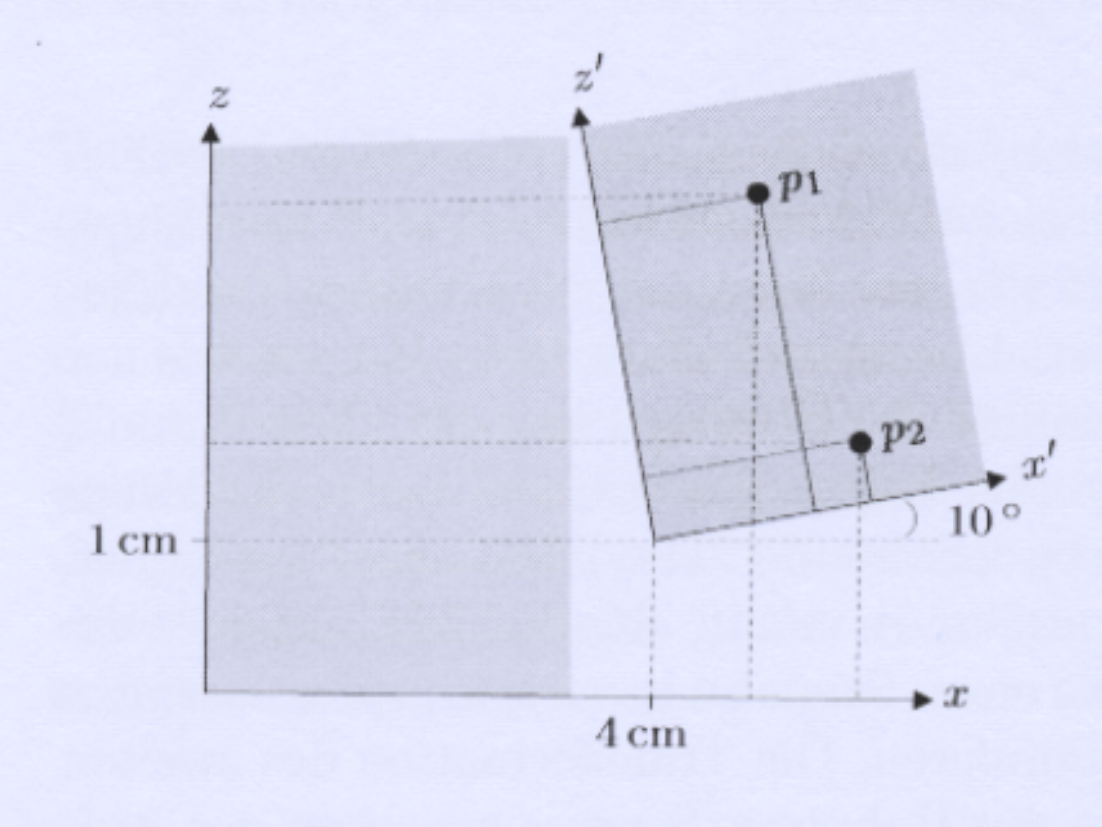
\includegraphics[scale=0.3]{Resources/PNG/2DScan.PNG}
		\caption{}
		\label{fig:PNG/2DScan.PNG}
	\end{center}
\end{figure}	
\begin{itemize}
	\item \textbf{Annahme:} die korrespondierenden Punkte sind bekannt $\Rightarrow$ eine \textbf{Transformation} kann berechnet werden, die diese Mengen aufeinander abbildet
	\item \textbf{Beispiel} zwei Scans mit einer Poseänderung des zweiten um $(4cm, 1cm, 10 \deg)^T$ beide Scans sehen dieselben Raumpunkte p1 und p2
	\item Obige Annahme i.d.r. nicht erfüllt $\Rightarrow$ \textbf{nicht eindeutig zu bestimmen, welche Punkte zwischen den beiden Scans korresponideren}
	\item \textbf{Lösung}: \textbf{iteratives Vorgehen}, bei dem zunächst eine \textbf{Schätzung} der Punktepaarung stattfinden und die Pose des zweiten Scans unter dieser Paarung optimiert wird.
	\item Iterativ werden mit dem transformierten Scan neue Punktepaare berechnet, bis ein Abbruchkriterium erfüllt ist, d.h. bis sich die Transformation zwischen zwei Schritten nich mehr signifikant ändert
\end{itemize}
\paragraph{Transformationsberechnung}
\begin{itemize}
	\item \textbf{Gesucht}: Mögliche Menge von Translationen und Rotationen, unter denen ein korrektes Matching möglich ist.
	\item $(t_x, t_z, \theta)^T$, die eine Translation um $t_x$ in x-Richtung und $t_z$ entlang der Z-Achse durchführt, sowie eine Rotation um den Winkel $\theta$
	\item Der Scan M besteht aus einer Menge von Punkten ($m_i$)i=1,2...N
	\item Der Scan D besteht aus einer Menge von Punkten ($D_i$)i=1,2...N
\end{itemize}
\paragraph{Minimum der Funktion}
$E(\theta, t)=\sum_{i=1}^{N}\left\|p_{i}-\left(\boldsymbol{R}_{\theta} \boldsymbol{p}_{i}^{\prime}+\boldsymbol{t}\right)\right\|^{2}$
\paragraph{Transformation zur mimierung der Fehlerfunktion E}
Folgende Transformation mit ggb. Parametern minimiert die Fehlerfunktion:\\
$\theta=\arctan \left(\frac{S_{z x^{\prime}}-S_{x z^{\prime}}}{S_{x x^{\prime}}+S_{z z^{\prime}}}\right)$
\\
Hierbei ist \\
$t_{x}=c_{x}-\left(c_{x}^{\prime} \cos \theta-c_{z}^{\prime} \sin \theta\right)$ und \\
$t_{z}=c_{z}-\left(c_{x}^{\prime} \sin \theta+c_{z}^{\prime} \cos \theta\right)$
%TODO Look at BSP 26 / 28






% Abbildungsverzeichnis generieren.
\clearpage
\addcontentsline{toc}{chapter}{\listfigurename}
\listoffigures

% Tabellenverzeichnis generieren.
%\clearpage
%\addcontentsline{toc}{chapter}{\listtablename}
%\listoftables

% Listingverzeichnis generieren.
\clearpage
%\renewcommand{\lstlistlistingname}{Listingverzeichnis}
\addcontentsline{toc}{chapter}{\lstlistlistingname}
\lstlistoflistings

\end{document}
